This project works on a layered data stack, that handles Big Data, i.e. large volumes of various structured and unstructured data types at a high velocity. The data stack handles how data is stored, managed, and retrieved to enable applications built on top of it. 
As there is no single data architecture that is generally accepted, i.e. different approaches use different architectures \cite{framptonCompleteGuideOpen2018,sakrBigDataProcessing2017}, thus this project defines a data stack, then focuses on improving its parts, namely the query engine. The data stack of the project is illustrated in Figure \ref{fig:data_stack}.

\begin{figure}[!ht]
    \begin{center}
      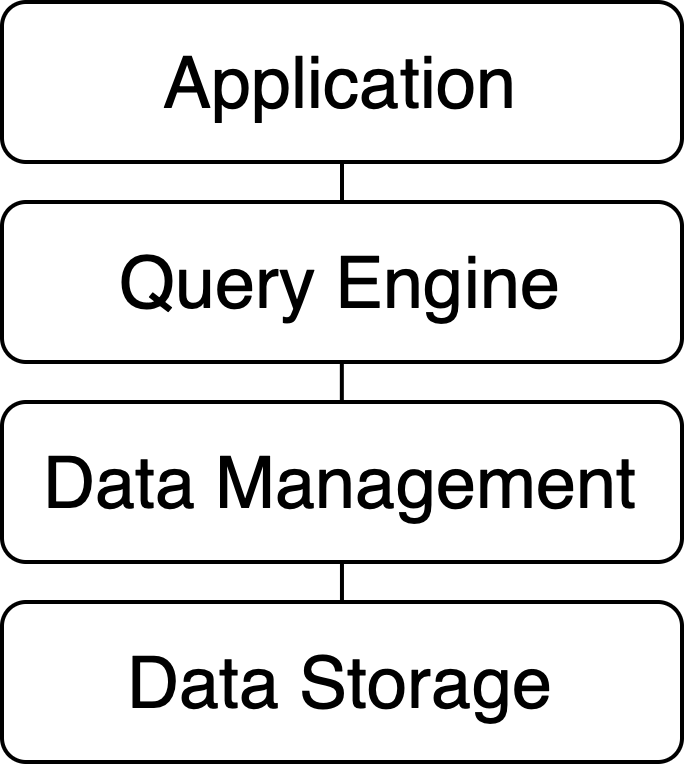
\includegraphics[width=0.4\textwidth]{figures/2-background/data_stack.png}
    \end{center}
    \caption{Data stack abstraction for this project}
    \label{fig:data_stack}
\end{figure}

The data stack (and this chapter) is divided into four sections:
\begin{enumerate}
    \item \textbf{Data Storage}: handles how the data is stored. The data storage layer might be centralized or distributed, on-premise or on the cloud, storing data in files, objects, or blocks.
    \item \textbf{Data Management} : handles how the data is managed. The data management layer might offer \gls{ACID} properties, data versioning, support open data formats, and/or support structured and/or unstructured data.
    \item \textbf{Query Engine}: handles how data is queried, i.e. accessed, retrieved and written. The query engine might offer caching, highly scalable architectures, and/or \gls{API} support for multiple programming languages.
    \item \textbf{Application}: a system that will take advantage of the data stack. In the case of this project, only the software of the host organization (Hopsworks' Feature Store) will be described. 
\end{enumerate}

After explaining the data stack, a section on programming languages complements the Background by explaining the roles different programming languages play in the data stack (namely, Python, Java, Scala, and Rust).
